\documentclass[a4j]{jarticle}
    \usepackage[dvipdfmx]{graphicx}
    \usepackage[ top=25truemm,bottom=25truemm,left=25truemm,right=25truemm]
    {geometry}
    \usepackage{ascmac}
    \usepackage{array}
    \usepackage{here}
    \usepackage{url}
    \usepackage{listings, jlisting}
    \renewcommand{\lstlistingname}{リスト}
\lstset{language=c,
  basicstyle=\ttfamily\scriptsize,
  commentstyle=\textit,
  classoffset=1,
  keywordstyle=\bfseries,
  frame=tRBl,
  framesep=5pt,
  showstringspaces=false,
  numbers=left,
  stepnumber=1,
  numberstyle=\tiny,
  tabsize=4
}

\makeatletter
\def\@thesis{プログラミング演習 レポート}
\def\id#1{\def\@id{#1}}
\def\department#1{\def\@department{#1}}

\def\@maketitle{
\begin{center}
{\huge \@thesis \par} %修士論文と記載される部分
\vspace{10mm}
{\LARGE\bf \@title \par}% 論文のタイトル部分
\vspace{10mm}
{\Large \@date\par}	% 提出年月日部分
\vspace{20mm}
{\Large \@department \par}	% 所属部分
{\Large 学籍番号 \@id \par}	% 学籍番号部分
\vspace{10mm}
{\Large 氏名 \@author}% 氏名 
\end{center}
\par\vskip 1.5em
}

\title{ミニゲーム}
\date{提出期限 2021年1月18日 17:00}
\department{組番号 408}
\id{17406}
\author{金澤雄大}

    \begin{document}
    \maketitle
    \thispagestyle{empty}
    \clearpage
    \addtocounter{page}{-1}
    \section{目的}
    後期のプログラミング演習で学習した内容の理解度を高めるために,ミニゲームを作成することを目的とする.
    \section{ゲームの説明}
    ゲームとして,「桃太郎電鉄」\cite{mmtt}(以下,桃鉄)をイメージした「ちゃま鉄」を作成した.「ちゃま鉄」は鉄道会社の運営をイメージしたすごろく形式のゲームである.
    本ゲームは,3年決戦で3人でのプレイを想定している.舞台設定は長野県である.プレイヤー(社長と呼ぶ)の目的は,3年経過時に自分の「総資産」を他の社長よりも多くすることである.\\
     総資産を増やす方法を説明する前に,ゲームの進行について説明する.ゲームスタート時に目的地がランダムに設定され,すべての社長に「所持金」として1億円が配られる.
    各社長は自分のターンにサイコロをふり,出た目の数だけ好きな方向に進めことができる.停車した駅には次に示す種類がある.マイナス駅で借金を背負った場合の処理はプログラムの説明の章で
    行う.
    \begin{itemize}
      \item プラス駅 $\dots$ 停車するとお金がもらえる駅
      \item マイナス駅 $\dots$ 停車するとお金が減る駅
      \item 物件駅 $\dots$ 停車すると物件を購入することができる駅
      \item 目的地駅 $\dots$ 特別な物件駅.停車するとお金がもらえ,物件を購入することができる駅
    \end{itemize}
     総資産は,物件駅に停車して物件を購入することで増やすことができる.物件駅とは図\ref{bukken_exsample}に示すように,その地域の
    名産品や観光地を購入できる駅のことである.図\ref{bukken_exsample}の長野駅の場合,6個の物件がある.物件にはそれぞれ「物件名」,「価格」,「収益率」の
    3つが設定されている.図\ref{bukken_exsample}の「りんごえん」の場合は物件名が「りんごえん」,価格が「600万円」,収益率が「120\%」である.
    所持金で購入できる物件は黒字,購入できない物件は赤字で表示される.図\ref{bukken_exsample}では所持金で購入できる「りんごえん」,
    「やわたやいそごろう」,「アイススケートじょう」が黒字,「ぜんこうじ」と「ながのこうせん」が赤字で表示されている.同じ駅の全ての
    物件を購入すると「独占」と呼ばれる状態になる.
    \begin{figure}[H]
      \centering
      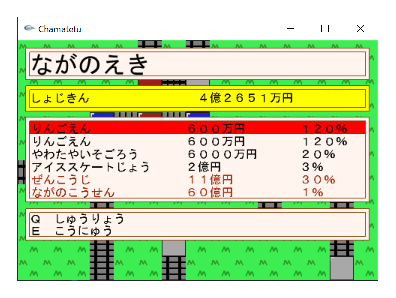
\includegraphics[scale=1.4]{bukkenex.eps}
      \caption{物件の例(長野駅)}
       \label{bukken_exsample}
      \end{figure}
    
      次に年月の仕様について説明する.ゲームスタート時は「1年目4月」に設定されている.プレイヤー3人のターンが1回終了すると
      1ヵ月が経過し,「1年目3月」が終了すると「2年目4月」になる.さらに,年月とは別に次に示すような季節の設定がある.
      ゲームの背景,プラス駅,マイナス駅の3つは季節によって変化する.ゲームの背景は季節にあったもの(例えば冬は雪が積もる)が描画される.プラス駅は
      夏は億単位のお金がもらえ,冬は百万円単位のお金しかもらえないという仕様になっている.マイナス駅は夏は百万円単位のお金しか減額されてないが,
      冬は億単位で減額される仕様になっている.この仕様は本家である桃鉄を参考にした.
      \begin{itemize}
      \item 春 : 3月~5月 
      \item 夏 : 6月~8月 
      \item 秋 : 9月~11月 
      \item 冬 : 12月~2月 
    \end{itemize}
       プラス駅と目的地駅でしかお金がもらえないと頻繁に金欠状態になってしまうため3月が終了すると「決算」が行われ,総資産に応じたお金が手に入る.
      決算でもらえるお金の計算方法について説明する.物件を$n$個持っているとき,決算でもらえる金額$S$は,所持している$i$番目の物件の価格$p_i$,収益率$r_i$,その物件が所属する
      駅が自分の独占のとき$d_i=2$,独占でないとき$d_i=1$とする変数を用いると式(\ref{kessan})のように表せる.
      \begin{equation}
        S = \sum_{i=1}^{n} \frac{p_i r_i d_i}{100}
        \label{kessan}
      \end{equation}

        例えば,ある社長が,図\ref{bukken_exsample}の「やわたやいそごろう」と「アイススケートじょう」を所持している場合に
      決算でもらえる金額を計算してみる.実際に計算すると式(\ref{kessan_ex1})のように1800万円になる.この例では独占はしていないから$d_i$は常に1である.
      \begin{eqnarray}
        S &=& \sum_{i=1}^{n} \frac{p_i r_i d_i}{100} \\
          &=& \frac{1}{100} \left( 6000\times10^4 \cdot 20 + 20000\times10^4 \cdot 3 \right) \\
          &=& 1800 \times10^4
        \label{kessan_ex1}
      \end{eqnarray}    

    \section{実行環境とビルド方法}
    本章では,実行環境およびビルド方法について述べる.
    \subsection{実行環境}
    実行環境を\ref{env}に示す.gccとは「GNU Compiler Collection」の略称で,GNUプロジェクトが公開しているコンパイラのことである.
    makeはMakefileにプログラムのコンパイルやリンクの方法を指示することで,コンパイルを簡単に行うことができるツールのことである.
    makeを用いることは,gccコンパイル時に,長いオプションを入力しなくてよい,ファイルの更新を取得して必要なものだけをコンパイルしてくれる
    という利点がある.

    \begin{table}[H]
      \caption{実行環境}
    \label{env}
    \begin{center}
        \begin{tabular}{c|l}\hline
          CPU & Intel(R) Core(TM) i7-6500U 2.50GHz  \\ 
          メモリ & 16.0GB DDR4 \\
          OS & Microsoft Windows 10 Home \\
          gcc &  version 9.3.0 \\
          make & version 4.3 \\ \hline
        \end{tabular}
    \end{center}
    \end{table}

    \subsection{ビルド方法}
    !

    \section{プログラムと実行結果}
    本章では,ゲームの実装部分について説明する.
    \subsection{構造体の定義と初期化}
    本ゲームを実装するうえで,プレイヤーや物件の情報を格納する方法として構造体を用いた.本節では次の3つの構造体の定義
    および初期化と値の格納について述べる.
    \begin{enumerate}
      \item playerstatus構造体
      \item propertystatus構造体
      \item stationstatus構造体
    \end{enumerate}

    \subsubsection{playerstatus構造体}
    playerstatus構造体は一人の社長の情報を保持するための構造体である.リスト\ref{playerstatus}に「game.h」におけるplayerstatus構造体の
    定義を示す. playerstatus構造体は「社長名」,「所持金」,「総資産」,「現在の座標(x,y)」の5つをメンバとして持っている.
    所持金および総資産は万円単位で扱うものとする.例えば所持金が「2200万円」場合,メンバmoneyには2200が代入される.これ以降にも金額を
    扱うための変数が登場するが,そのすべての変数は万円単位で扱うものとする.
    11行目のようにplayerstatus構造体の配列を定義することで,プレイ人数3人分の情報を保持する構造体の配列を作成している.
    \begin{lstlisting}[basicstyle=\ttfamily\footnotesize, frame=single,label=playerstatus,caption=playerstatus構造体の定義と初期化]
// プレイヤーの情報構造体
struct playerstatus{
    char name[NAMEMAX]; // 社長名
    int money; // 所持金
    int assets; // 総資産
    int x; // x座標(実描画座標)
    int y; // y座標(実描画座標)
};

typedef struct playerstatus player;
player players[PLAYERNUM]; // 人数分の配列を確保
    \end{lstlisting}

    \subsubsection{propertystatus構造体}
    propertystatus構造体は一つの物件の情報を保持するための構造体である.「game.h」におけるpropertystatus構造体の定義をリスト\ref{propertystatus}に示す.
     propertystatus構造体は「物件名」,「物件保持者」,「価格」,「収益率」の4つをメンバとして持っている.物件保持者は表\ref{whohold}のルールで扱うものとする.
    \begin{lstlisting}[basicstyle=\ttfamily\footnotesize, frame=single,label=propertystatus,caption=propertystatus構造体の定義]
// 物件情報構造体
struct propertystatus{
    char name[STRMAX]; // 物件名
    int holder; // 物件所持者
    int price; // 価格
    int earnings; // 収益率
};

typedef struct propertystatus property;
    \end{lstlisting}

    \begin{table}[H]
      \caption{物件保持者メンバの意味}
    \label{whohold}
    \begin{center}
        \begin{tabular}{c|c}\hline
        値 & 保持者 \\ \hline \hline
          0 & 保持者なし \\
          1 & 社長1 \\
          2 & 社長2 \\
          3 & 社長3 \\ \hline
        \end{tabular}
    \end{center}
    \end{table}

    \subsubsection{stationstatus構造体}
    stationstatus構造体は一つの駅の情報を保持するための構造体である.リスト\ref{stationstatus}にstationstatus構造体の定義を示す.
    stationstatus構造体は,「駅名」,「駅の座標(x,y)」,「独占フラグ」,「物件の数」,「propertystatus構造体の配列」の6つをメンバとして持つ.
    駅の座標(x,y)はplayerstatus構造体のような実座標ではなく,マップを描画するための配列の番号である.詳細については!で述べる.独占フラグは
    その駅を誰が独占しているかを判別するために用いる.独占フラグの値とその意味は表\ref{whohold}と同じである.
    \begin{lstlisting}[basicstyle=\ttfamily\footnotesize, frame=single,label=stationstatus,caption=stationstatus構造体の定義と初期化]
// 駅情報構造体
struct stationstatus{
    char name[STRMAX]; // 駅名
    int x; // x座標
    int y; // y座標
    int ismonopoly; // 独占フラグ
    int propertynum; // 物件数
    property plist[PROPERTMAX]; // 物件情報構造体の配列
};

typedef struct stationstatus station;
station stations[STATIONNUM]; // 駅の数分の配列を確保
station distination; // 目的地配列
    \end{lstlisting}    

    \subsubsection{構造体への値の格納}
    構造体に値を格納するためのコードについて説明する.まず,playerstatus構造体の初期化について説明する.
    リスト\ref{InitPlayer}にInitPlayer関数および初期化を確認するためのdispPlayer関数のコードを示す.
    InitPlayer関数ではfor文を用いてplayerstatus構造体への値の格納を行っている.6行目で不思議な文字列を社長名のメンバに
    格納しているが,これは日本語を画面出力するための独自プロトコルでの「プレイヤー1」という表現である.日本語プロトコルの
    説明については!で行う.dispPlayer関数はplayerstatus構造体に値が格納されていることを確認するための関数である.
    引数として0を与えるとすべての社長のメンバ情報を表示する.引数として1,2,3のいずれかを与えると表\ref{whohold}に対応した
    社長のメンバ情報だけを表示する.
    \begin{lstlisting}[basicstyle=\ttfamily\footnotesize, frame=single,label=InitPlayer,caption=playerstatus構造体への値の格納]
// 画像サイズ
#define IMGSIZE 32
// 初期プレイヤー座標
#define INITX 13*IMGSIZE
#define INITY 7*IMGSIZE
// 初期所持金
#define INITMONEY 10000

// プレイヤー構造体を初期化
void InitPlayer(void){
    int i;
    for(i=0;i<PLAYERNUM;i++){
        //プレイヤーhoge
        sprintf(players[i].name,"llpureiiyallms%d",i+1);
        players[i].x=INITX;
        players[i].y=INITY;
        players[i].money=INITMONEY;
        players[i].assets=0;
    }
}

// デバッグ用関数 	
// プレイヤー構造体を表示	
// detail : 0 全部表示 , else その番号の駅を表示	
void dispPlayer(int detail){	
    int i;	
    if(detail==0){	
        for(i=0;i<PLAYERNUM;i++){	
            printf("--------------------\n");	
            printf("%s社長 (%d,%d)\n",players[i].name,players[i].x,players[i].y);	
            printf("\n");	
            printf("所持金 : %d\n",players[i].money);	
            printf("総資産 : %d\n",players[i].assets);	
            printf("--------------------\n\n");	
        }	
    }else{	
        printf("--------------------\n");	
        printf("%s社長 (%d,%d)\n",players[detail-1].name,
        players[detail-1].x,players[detail-1].y);	
        printf("\n");	
        printf("所持金 : %d\n",players[detail-1].money);	
        printf("総資産 : %d\n",players[detail-1].assets);	
        printf("--------------------\n\n");   	
    }	
}
          \end{lstlisting}        

    リスト\ref{InitPlayerCheck}のコードを実行して,構造体に値が代入されていることを確認する.必要なヘッダファイルについては付録を参照してほしい.
    正しく実行できていれば,座標(x,y)は(416,224),所持金は10000,総資産は0になるはずである.リスト\ref{InitPlayerResult}にリスト\ref{InitPlayerCheck}のコードの実行結果を示す.
    リスト\ref{InitPlayerResult}から,座標,所持金,総資産がすべての社長について正しい値であることがわかる.これよりplayerstatus構造体の定義および初期化の方法が
    確認できた.
    \begin{lstlisting}[basicstyle=\ttfamily\footnotesize, frame=single,label=InitPlayerCheck,caption=InitPlayer関数の動作確認]
int main(int argc, char **argv){
    InitPlayer();
    dispPlayer(0);
}
  \end{lstlisting}   

  \begin{lstlisting}[basicstyle=\ttfamily\footnotesize, frame=single,label=InitPlayerResult,caption=リスト\ref{InitPlayerCheck}の実行結果]
--------------------
llpureiiyallms1社長 (416,224)

所持金 : 10000
総資産 : 0
--------------------

--------------------
llpureiiyallms2社長 (416,224)

所持金 : 10000
総資産 : 0
--------------------

--------------------
llpureiiyallms3社長 (416,224)

所持金 : 10000
総資産 : 0
--------------------
      \end{lstlisting} 
      
    次に,駅の情報および物件の情報を構造体に格納する方法について説明する.駅の情報はリスト\ref{propertytxt}に示すproperty.txtに
    記述されている. property.txtには各駅について「駅名」,駅の座標(x,y)が記述されている.駅名は独自の日本語プロトコルで記述されている.
    \begin{lstlisting}[basicstyle=\ttfamily\footnotesize, frame=single,label=propertytxt,caption=property.txt]
nozawaoonnsenn 18,1
iiiiyama 13,3
togakusi 9,9
nagano 13,7
oobuse 19,7
suzaka 19,11
matusiro 12,10
sinonoii 9,12
hakuba 3,7
oooomati 3,18
tikuma 9,15
uueeda 19,15
karuiizawa 23,15
aadumino 3,20
saku 23,18
matumoto 9,22
suwa 17,25
kiso 3,25
ookaya 9,27
iiiida 20,28
iina 23,27
            \end{lstlisting}    
    
    駅の情報はproperty.txtをファイル読み込みによって行う. 駅の情報を読み込むための関数であるreadStation関数のコードを
    リスト\ref{readStation}に示す.リスト\ref{readStation}において読み取った値をstationstatus構造体に代入しているのは
    11行目から14行目である.11行目でfscanf関数を用いて「駅名 x座標,y座標」という情報を読み取って構造体に代入している.
    \begin{lstlisting}[basicstyle=\ttfamily\footnotesize, frame=single,label=readStation,caption=readStation関数のコード]
// ファイルから駅情報を取得
// stations構造体を初期化
void readStation(void){
    FILE *fp;
    int i=0;
    fp=fopen("property.txt","r");
    if(fp==NULL){ // 開けなかったとき
        printf("file not found");
        exit(0);
    }else{ // 駅名と座標を取得
        while(fscanf(fp,"%s %d,%d",stations[i].name,&stations[i].x,&stations[i].y)!=EOF){
            stations[i].ismonopoly=0; // 独占フラグ初期化
            i++;
        }
        fclose(fp);
    }
}
        \end{lstlisting}      

    物件情報も同様にファイルから読み込む仕様にした.物件情報は「/property」に「駅名.txt」という形で保存している.
    リスト\ref{naganotxt}およびリスト\ref{matumototxt}に物件情報を保存しているファイルの例を示す.リスト\ref{naganotxt}は
    長野駅,リスト\ref{matumototxt}は松本駅である.どちらの場合も,物件の情報は「物件名 価格,収益率」という形式で保存している.
    \begin{lstlisting}[basicstyle=\ttfamily\footnotesize, frame=single,label=naganotxt,caption=/property/nagano.txt]
rinngoeenn 600,120
rinngoeenn 600,120
yawatayaiisogorouu 6000,20 
llaaiisusukellmslltollzilouu 20000,3 
zennkouuzi 110000,30
naganokouusenn 600000,1
    \end{lstlisting}  

    \begin{lstlisting}[basicstyle=\ttfamily\footnotesize, frame=single,label=matumototxt,caption=/property/matumoto.txt]
giluuuniluuullpannll 1200,130 
kamikouuti 12000,80
sinnsiluuudaiigaku 60000,30
aasamaoonnsenn 80000,4
kiluuukaiitigaltkouu 90000,5
matumotozilouu 150000,5
    \end{lstlisting}     

    リスト\ref{readProperty}にファイルから物件情報を取得するための関数であるreadProperty関数,および読み込めたことを確認するためのdispStation関数
    のコードを示す.readProperty関数においてファイルから物件の情報を読み込んでいるのは15行目から19行目である.readStation関数同様に,fscanf関数を用いて
    一行ずつ物件情報を読み取ってpropertystatus構造体に代入している.dispStation関数の仕様もdispPlayer関数と同様である.引数として0を与えると
    すべての駅の情報が標準出力され,1,2$\dots$という番号を与えると,対応したインデックスの駅情報のみが出力される.
    \begin{lstlisting}[basicstyle=\ttfamily\footnotesize, frame=single,label=readProperty,caption=readProperty関数とdispStation関数]
// ファイルから物件情報を取得
void readProperty(void){
    FILE *fp;
    int i,j;
    char fname[100];
    for(i=0;i<STATIONNUM;i++){
        sprintf(fname,".\\property\\%s.txt",stations[i].name);
        fp=fopen(fname,"r");
        j=0;
        if(fp==NULL){ // 開けなかったとき
            printf("file not found in %s",stations[i].name);
            exit(0);
        }else{
            // 物件名,値段,収益率を取得
            while(fscanf(fp,"%s %d,%d",stations[i].plist[j].name,
            &stations[i].plist[j].price,&stations[i].plist[j].earnings)!=EOF){
            stations[i].plist[j].holder=0; // 購入フラグ初期化
            j++;
        }
        stations[i].propertynum=j; // 物件数を保存
        fclose(fp);
    }

    }   
}

// デバッグ用関数	
// 駅情報を表示	
void dispStation(int detail){	
    int i,j;	
    if(detail==0){	
        for(i=0;i<STATIONNUM;i++){	
            printf("--------------------\n");	
            printf("%s駅 (%d,%d)\n",stations[i].name,stations[i].x,stations[i].y);	
            printf("独占フラグ : %d   物件数 : %d\n",stations[i].ismonopoly,
            stations[i].propertynum);	
            for(j=0;j<stations[i].propertynum;j++){	
                printf("%s %d %d %d\n",stations[i].plist[j].name,
                stations[i].plist[j].price,stations[i].plist[j].earnings,
                stations[i].plist[j].holder);	
            }	
            printf("--------------------\n\n");	
        }	
        }else{	
        printf("--------------------\n");	
        printf("%s駅 (%d,%d)\n",stations[detail-1].name,stations[detail-1].x,
        stations[detail-1].y);	
        printf("独占フラグ : %d   物件数 : %d\n",stations[detail-1].ismonopoly,
        stations[detail-1].propertynum);	
        for(j=0;j<stations[detail-1].propertynum;j++){	
            printf("%s %d %d %d\n",stations[detail-1].plist[j].name,
            stations[detail-1].plist[j].price,
            stations[detail-1].plist[j].earnings,
            stations[detail-1].plist[j].holder);	
        }	
        printf("--------------------\n\n");     	
    }	
}
    \end{lstlisting} 

    リスト\ref{readCheck}に駅および物件の情報が正常に読み込まれ,構造体に格納されていることを確認するコードを示す.正しく実行できていれば,
    ファイルから読み取った駅および物件の情報が表示されるはずである.リスト\ref{readCheck}にリスト\ref{readCheck}のコードの実行結果を示す.
    実行結果として21駅分の結果を載せると長くなるため,ここでは必要な駅のみを載せることにする.リスト\ref{readCheck}から,リスト\ref{propertytxt}
    の一番目の野沢温泉駅から,末尾の伊那駅まで全ての駅が読み込まれていることを確認した.また,例として掲載した長野駅および松本駅について,
    ファイルに記述した情報と標準出力した情報に違いがないことが確認できる.これらより,ファイルから駅および物件の情報を読み込み,構造体に格納できていることが
    確認できた.
    \begin{lstlisting}[basicstyle=\ttfamily\footnotesize, frame=single,label=readCheck,caption=駅および物件読み込みの動作確認]
int main(int argc, char **argv){
    readStation();
    readProperty();
    dispStation(0);
}
          \end{lstlisting} 

    \begin{lstlisting}[basicstyle=\ttfamily\footnotesize, frame=single,label=readResult,caption=リスト\ref{readCheck}の実行結果]
--------------------
nozawaoonnsenn駅 (18,1)
独占フラグ : 0   物件数 : 6
nozawanaoyaki 3000 80 0
nozawanaoyaki 3000 80 0
nozawanaoyaki 3000 80 0
ooooyu 12000 5 0
llsukillmszilouu 40000 10 0
llsukillmszilouu 40000 10 0
--------------------

(中略)

--------------------
nagano駅 (13,7)
独占フラグ : 0   物件数 : 6
rinngoeenn 600 120 0
rinngoeenn 600 120 0
yawatayaiisogorouu 6000 20 0
llaaiisusukellmslltollzilouu 20000 3 0
zennkouuzi 110000 30 0
naganokouusenn 600000 1 0
--------------------

(中略)

--------------------
matumoto駅 (9,22)
独占フラグ : 0   物件数 : 6
giluuuniluuullpannll 1200 130 0
kamikouuti 12000 80 0
sinnsiluuudaiigaku 60000 30 0
aasamaoonnsenn 80000 4 0
kiluuukaiitigaltkouu 90000 5 0
matumotozilouu 150000 5 0
--------------------

(中略)

--------------------
iina駅 (23,27)
独占フラグ : 0   物件数 : 3
rinngollpaiill 3000 75 0
bunnguiitouuge 30000 7 0
takatooozilouusi 130000 5 0
--------------------
          \end{lstlisting} 

    \subsection{メイン関数}
    メイン関数について説明する.リスト\ref{main}にメイン関数のコードを示す.
    メイン関数の処理について説明する.リスト\ref{main}の12行目および13行目ではウィンドウの生成を行っている.
    本ゲームではウィンドウサイズは480$\times$320の固定サイズとする.22行目から25行目では,画像の読み込みおよび
    構造体の初期化を行っている.28行目から31行目ではコールバック関数の登録を行っている.これによって,キーボード入力
    やウィンドウのサイズ変更といったイベントが発生したときに,そのイベントに対応した関数が呼び出されて,処理が
    行われる.
    \begin{lstlisting}[basicstyle=\ttfamily\footnotesize, frame=single,label=main,caption=メイン関数]
#include <GL/glut.h>
#include <GL/glpng.h>
#include <stdio.h>
#include <stdlib.h>
#include <time.h>
#include "game.h"

int main(int argc, char **argv)
{
    srand((unsigned) time(NULL));
    glutInit(&argc, argv);
    glutInitWindowSize(InitWidth,InitHeight);
    glutCreateWindow("Chamatetu");
    glutInitDisplayMode(GLUT_RGBA | GLUT_ALPHA);
    glClearColor(1.0, 1.0, 1.0, 0.0);

    //  テクスチャのアルファチャネルを有効にする設定
    glEnable(GL_BLEND);
    glBlendFunc(GL_SRC_ALPHA, GL_ONE_MINUS_SRC_ALPHA);
    glTexEnvf(GL_TEXTURE_ENV, GL_TEXTURE_ENV_MODE, GL_MODULATE);
    
    readImg();
    InitPlayer();
    readStation();
    readProperty();
    turnstatus=0;
    //イベント登録
    glutReshapeFunc(Reshape);
    glutDisplayFunc(Display);
    glutKeyboardFunc(keyboard);
    glutTimerFunc(RESHAPETIME, Timer, 0);
    //  イベントループ突入
    glutMainLoop();

    return(0);
}
                  \end{lstlisting}     
    
    \subsection{日本語の表示方法}
    本節では日本語を表示する方法について,次に示す内容を述べる.
    !
    \subsubsection{日本語プロトコルの説明}
    桃鉄をイメージしたゲームを実装するうえで,日本語を画面に表示できなければ,ローマ字が並んでわかりにくい.しかしGLUTは日本語に対応していない.
    そこで画像を用いて日本語をゲーム画面に描画する機能を作成した.これを日本語プロトコルと呼ぶことにする.文字色については黒と赤のどちらかで描画することが可能である.
    作成した日本語プロトコルでは次に示す文字を画面に表示することができる.一部のアルファベット,記号,漢字をまとめて特殊文字と呼ぶことにする.
    \begin{itemize}
      \item 50音(ひらがな,カタカナ)
      \item 濁音(ひらがな,カタカナ)
      \item 半濁音(ひらがな,カタカナ)
      \item 小文字(っ,ゃ,ゅ,ょ)(ひらがな,カタカナ)
      \item 数字
      \item 一部のアルファベット(W,A,S,D,E,Q)
      \item 一部の記号(読点,句点,\%,マイナスの記号(-),プラスの記号(+))
      \item ゲームに頻出する漢字(億,万,円)
    \end{itemize}

    これらの画像は「/charimg」に保存されている.画像のサイズはすべて32$\times$32pxである.画像名の意味は図\ref{howname}の通りである.
    どの文字か判別する2文字はコード中で日本語を表示するための文字列に対応している.実際の文字と日本語プロトコルにおける文字の表現
    方法は表\ref{jpp}の通りである.改行およびスペースは画像にはないが,画像を表示する位置を調整することで表現できる.表\ref{jpp}の情報は
    game.cでリスト\ref{jpProtcolarray}に示すように定義されている.
    
    \begin{figure}[H]
      \centering
      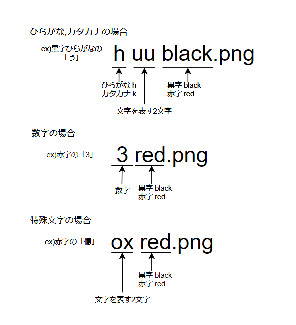
\includegraphics[scale=1.7]{howname.eps}
      \caption{画像の名前の意味}
       \label{howname}
      \end{figure}    

      \begin{table}[H]
        \caption{日本語プロトコルの文字表現}
      \label{jpp}
      \begin{center}
          \begin{tabular}{c|c|c|c|c}\hline
あ aa & い ii & う uu & え ee & お oo \\ 
か ka & き ki & く ku & け ke & こ ko \\ 
さ sa & し si & す su & せ se & そ so \\ 
た ta & ち ti & つ tu & て te & と to \\ 
な na & に ni & ぬ nu & ね ne & の no \\ 
は ha & ひ hi & ふ hu & へ he & ほ ho \\ 
ま ma & み mi & む mu & め me & も mo \\ 
や ya & -  & ゆ yu & -  & よ yo \\ 
ら ra & り ri & る ru & れ re & ろ ro \\ 
わ wa & -  & を wo & -  & ん nn \\ 
ゃ la & - & ゅ lu & っ lt & ょ lo \\ 
が ga & ぎ gi & ぐ gu & げ ge & ご go \\ 
ざ za & じ zi & ず zu & ぜ ze & ぞ zo \\
だ da & ぢ di & づ du & で de & ど do \\
ば ba & び bi & ぶ bu & べ be & ぼ bo \\ 
ぱ pa & ぴ pi & ぷpu &  ぺ pe & ぽ po \\ 
0  0 & 1  1 & 2  2 & 3  3 & 4  4 \\ 
5  5 & 6  6 & 7  7 & 8  8 & 9  9 \\ 
円 ex & 万 mx & 億 ox & \% px & - ms \\ 
+ ps & 句点 mr & 読点 tn & Q xq & W xw \\ 
E xe & A xa & S xs & D xd & - \\ 
改行 xx & スペース ss & - & - & - \\ \hline
          \end{tabular}
      \end{center}
      \end{table}
      
      \begin{lstlisting}[basicstyle=\ttfamily\footnotesize, frame=single,label=jpProtcolarray,caption=jpProtcol配列]
// 日本語プロトコル
char jpProtcol[JPMAX+SPMAX][3] = {"aa","ii","uu","ee","oo",
                            "ka","ki","ku","ke","ko",
                            "sa","si","su","se","so",
                            "ta","ti","tu","te","to",
                            "na","ni","nu","ne","no",
                            "ha","hi","hu","he","ho",
                            "ma","mi","mu","me","mo",
                            "ya","yu","yo",
                            "ra","ri","ru","re","ro",
                            "wa","wo","nn",
                            "lt","la","lu","lo",
                            "ga","gi","gu","ge","go",
                            "za","zi","zu","ze","zo",
                            "da","di","du","de","do",
                            "ba","bi","bu","be","bo",
                            "pa","pi","pu","pe","po",
                            "0","1","2","3","4","5"
                            ,"6","7","8","9",
                            "ex","mx","ox","px","ms","ps",
                            "mr","tn","xq","xw","xe","xa","xs","xd"
                            };

      \end{lstlisting} 
      \subsubsection{画像を読み込む方法}
      画像の読み込ム部分のコードをリスト\ref{readImg}に示す.画像の情報を格納する配列(リスト\ref{readImg}の3行目から30行目)はgame.hに定義してある.
      readImg関数はリスト\ref{readImg}の33行目から107行目である. readImg関数では日本語プロトコルのため画像,イベント用の画像,季節別背景の画像,
      マップの画像,プレイヤーの画像,サイコロの画像を読み込んでいる.画像名はsprintf関数を用いて指定し,画像をpngBind関数で読み込んでいる.
      \begin{lstlisting}[basicstyle=\ttfamily\footnotesize, frame=single,label=readImg,caption=readImg関数]
// 画像用変数
// 季節画像
GLuint seasonimg[SEASON_NUM];
pngInfo seasoninfo[SEASON_NUM];
// マップ画像
GLuint mapimg[MAP_NUM];
pngInfo mapinfo[MAP_NUM];
// プレイヤー画像
GLuint playerimg[PLAYERNUM];
pngInfo playerinfo[PLAYERNUM];
// サイコロ画像
GLuint diceimg[DICEMAX];
pngInfo diceinfo[DICEMAX];
// イベント画像
GLuint spimg[SP_NUM];
pngInfo spinfo[SP_NUM];

// 日本語画像
// ひらがな黒
GLuint hblackimg[JPMAX+SPMAX];
pngInfo hblackinfo[JPMAX+SPMAX];
// ひらがな赤
GLuint hredimg[JPMAX+SPMAX];
pngInfo hredinfo[JPMAX+SPMAX];
// カタカナ黒
GLuint kblackimg[JPMAX];
pngInfo kblackinfo[JPMAX];
// カタカナ赤
GLuint kredimg[JPMAX];
pngInfo kredinfo[JPMAX];

// 画像読み込み
void readImg(void){
    int i;
    char fname[100];

    // イベントマップ読み込み
    for(i=0;i<SP_NUM;i++){
        sprintf(fname,".\\eventparts\\sp%d.png",i+1);
        spimg[i] = pngBind(fname, PNG_NOMIPMAP, PNG_ALPHA, 
       &spinfo[i], GL_CLAMP, GL_NEAREST, GL_NEAREST);        
    }

   // 季節マップ読み込み 
    for(i=0;i<SEASON_NUM;i++){
        sprintf(fname,".\\mapparts\\season%d.png",i+1);
        seasonimg[i] = pngBind(fname, PNG_NOMIPMAP, PNG_ALPHA, 
       &seasoninfo[i], GL_CLAMP, GL_NEAREST, GL_NEAREST);        
    }

    // マップイメージ読み込み
    for(i=0;i<=MAP_NUM;i++){
        sprintf(fname,".\\mapparts\\map%d.png",i+1);
        mapimg[i] = pngBind(fname, PNG_NOMIPMAP, PNG_ALPHA, 
       &mapinfo[i], GL_CLAMP, GL_NEAREST, GL_NEAREST);
    }
    // プレイヤー画像を読み込み
    for(i=0;i<PLAYERNUM;i++){
        sprintf(fname,".\\eventparts\\player%d.png",i+1);
        playerimg[i] = pngBind(fname, PNG_NOMIPMAP, PNG_ALPHA, 
       &playerinfo[i], GL_CLAMP, GL_NEAREST, GL_NEAREST);
    }

    // サイコロの画像を読み込み
    for(i=0;i<DICEMAX;i++){
        sprintf(fname,".\\dice\\dice%d.png",i+1);
        diceimg[i] = pngBind(fname, PNG_NOMIPMAP, PNG_ALPHA, 
       &diceinfo[i], GL_CLAMP, GL_NEAREST, GL_NEAREST);
    }
    // read Hiragana black
    for(i=0;i<JPMAX;i++){
        sprintf(fname,".\\charimg\\h%sblack.png",jpProtcol[i]);
        hblackimg[i] = pngBind(fname, PNG_NOMIPMAP, PNG_ALPHA, 
        &hblackinfo[i], GL_CLAMP, GL_NEAREST, GL_NEAREST);
    }

    // read Hiragana red
    for(i=0;i<JPMAX;i++){
        sprintf(fname,".\\charimg\\h%sred.png",jpProtcol[i]);
        hredimg[i] = pngBind(fname, PNG_NOMIPMAP, PNG_ALPHA, 
        &hredinfo[i], GL_CLAMP, GL_NEAREST, GL_NEAREST);
    }
    // read Katakana black
    for(i=0;i<JPMAX;i++){
        sprintf(fname,".\\charimg\\k%sblack.png",jpProtcol[i]);
        kblackimg[i] = pngBind(fname, PNG_NOMIPMAP, PNG_ALPHA, 
        &kblackinfo[i], GL_CLAMP, GL_NEAREST, GL_NEAREST);
    }
    // read Katakana red
    for(i=0;i<JPMAX;i++){
        sprintf(fname,".\\charimg\\k%sred.png",jpProtcol[i]);
        kredimg[i] = pngBind(fname, PNG_NOMIPMAP, PNG_ALPHA, 
        &kredinfo[i], GL_CLAMP, GL_NEAREST, GL_NEAREST);
    }
    // read Special Str red
    for(i=JPMAX;i<JPMAX+SPMAX;i++){
        sprintf(fname,".\\charimg\\%sred.png",jpProtcol[i]);
        hredimg[i] = pngBind(fname, PNG_NOMIPMAP, PNG_ALPHA, 
        &hredinfo[i], GL_CLAMP, GL_NEAREST, GL_NEAREST);
    }
    // read Special Str black
    for(i=JPMAX;i<JPMAX+SPMAX;i++){
        sprintf(fname,".\\charimg\\%sblack.png",jpProtcol[i]);
        hblackimg[i] = pngBind(fname, PNG_NOMIPMAP, PNG_ALPHA, 
        &hblackinfo[i], GL_CLAMP, GL_NEAREST, GL_NEAREST);
    }
}
                  \end{lstlisting} 

      
    \subsubsection{画像を表示する関数}
    画像を表示するための関数としてPutSprite関数がある.この関数は授業中に使用した関数であるが,画像のサイズを変更できるように
    改造した.リスト\ref{PutSprite}にPutSprite関数のコードを示す.PutSprite関数は引数として受け取った座標(x,y)に
    倍率scaleで画像を描画する関数である.
    \begin{lstlisting}[basicstyle=\ttfamily\footnotesize, frame=single,label=PutSprite,caption=PutSprite関数]
// (x,y)に大きさscaleの画像を表示
void PutSprite(int num, int x, int y, pngInfo *info,double scale)
{
    int w, h;  //  テクスチャの幅と高さ

    w = info->Width*scale;   //  テクスチャの幅と高さを取得する
    h = info->Height*scale;

    glPushMatrix();
    glEnable(GL_TEXTURE_2D);
    glBindTexture(GL_TEXTURE_2D, num);
    glColor4ub(255, 255, 255, 255);

    glBegin(GL_QUADS);  //  幅w, 高さhの四角形

    glTexCoord2i(0, 0); 
    glVertex2i(x, y);

    glTexCoord2i(0, 1);
    glVertex2i(x, y + h);

    glTexCoord2i(1, 1);
    glVertex2i(x + w, y + h);

    glTexCoord2i(1, 0);
    glVertex2i(x + w, y);

    glEnd();

    glDisable(GL_TEXTURE_2D);
    glPopMatrix();
}
          \end{lstlisting}

    \subsubsection{文字列による画像の表示制御}
    1文字を描画する関数として,drawChar関数を作成した.リスト\ref{drawChar}にdrawChar関数のコードを示す.
    drawChar関数は引数として表示する文字のjpProtcol配列のインデックスnum,ひらがな/カタカナのどちらで描画するかを
    判別する変数kh,黒/赤のどちらで描画するかを判別する変数color,描画する座標(x,y),表示する大きさscaleを受け取る.
    変数khはひらがなのとき0,カタカナのとき1である.変数colorは黒のとき0,赤のとき1である.変数スケールは1のとき32$\times$32px
    で描画される.
    \begin{lstlisting}[basicstyle=\ttfamily\footnotesize, frame=single,label=drawChar,caption=drawChar関数]
// 1文字の日本語を表示
// int kh : 0,Hiragana 1,Katakana
// int color 0,black 1,red
void drawChar(int num,int kh,int color,int x,int y,double scale){
    if(kh==0){
        if(color==0){ // hiragana black
            PutSprite(hblackimg[num], x, y, &hblackinfo[num],scale);
        }else{ //hiragana red
            PutSprite(hredimg[num], x, y, &hredinfo[num],scale);
            }
        }else{ 
        if(color==0){ // katakana black
            PutSprite(kblackimg[num], x, y, &kblackinfo[num],scale);
        }else{ // katakana red
            PutSprite(kredimg[num], x, y, &kredinfo[num],scale);
        }
    }
}
                \end{lstlisting}

    1文字を描画するたびにdrawChar関数を呼び出すと大変だから,文字列を引数として渡すと自動で描画が行われる関数を作成した.リスト\ref{drawString}
    にdrawString関数のコードを示す.この関数を用いて実際に描画を行う例については,!節以降で説明する.
    drawString関数は引数として受け取った文字列stringを描画する関数である.文字列の他に引数として
    描画する色color,1文字目を表示する座標(xo,yo),表示する大きさscaleを受け取る.座標(xo,yo)は1文字目の左上の座標である.
    drawString関数の内部では,for文を用いて文字列stringの文字を1文字,または2文字ずつ取り出し,その文字が数字,日本語,特殊文字,スペース,改行の
    どれにあたるかチェックしている.該当する文字が発見された場合はdrawChar関数に配列の番号と描画位置の情報を渡して描画を行っている.
    1文字描画したら,次の文字を描画するために,描画する座標を計算する.これはリスト\ref{drawString}の40行目から43行目で行っている.
    \begin{lstlisting}[basicstyle=\ttfamily\footnotesize, frame=single,label=drawString,caption=drawString関数]
// 引数stringの文字列を表示
void drawString(char *string,int color,int xo,int yo,double scale){
    int i,j;
    int len = strlen(string);
    int x=xo;
    int y=yo;
    int flg;
    int kh=0;
    for(i=0;i<len;i++){
        flg=string[i]-'0'; // インデクス計算
        if((flg>=0)&&(flg<=9)){ // 数字描画
            drawChar(JPMAX+flg,0,color,x,y,scale);
            flg=1;
        }else{
            for(j=0;j<JPMAX;j++){ //日本語描画
                if((jpProtcol[j][0]==string[i])&&(jpProtcol[j][1]==string[i+1])){
                    drawChar(j,kh,color,x,y,scale);
                    break;
                }
            }       
            for(j=JPMAX+10;j<JPMAX+SPMAX;j++){ //特殊文字描画
                if((jpProtcol[j][0]==string[i])&&(jpProtcol[j][1]==string[i+1])){
                    drawChar(j,kh,color,x,y,scale);
                    break;
                }
            }
            flg=1;
            if((string[i]=='l')&&(string[i+1]=='l')){ //ひらがな/カタカナ切り替え
                kh=1-kh;
                flg=0;
            }
            if((string[i]=='x')&&(string[i+1]=='x')){ // 改行
                x=xo;
                flg=0;
                y+=IMGSIZE*scale;
            }     
            i++;
        }
        if(flg==1){ // 次の座標に移動
            x+=IMGSIZE*scale;
            if(x>InitWidth-22){
                x=xo;
                y+=IMGSIZE*scale;
            }
        }
    }
}
    \end{lstlisting}

    \subsection{Display関数によるゲームの状況制御}
    ゲームの進行処理は一括してDisplay関数で行っている.Display関数のコードは行数があるため,
    付録に掲載する.ゲームの進行状況にはturnstatusとinflgという2つの変数を用いている.
    変数turnstatusは今どの処理を行っているのかを大きな区分で表すための変数である.変数inflgは
    各turnstatusの中で,詳細な処理(例えばダイアログを表示する,タイマーを起動する)を行うための変数である.
    ゲームの進行状況とturnstatusの値の関係を表\ref{turnstatus}に示す.turnstatusの10~14が欠番になっているのは,
    開発時間の都合上作成できなかったカード処理のために予約しておいた番号のためである.それぞれのturnstatusでの処理は
    次節以降で説明する.turnstatusはメイン関数(リスト\ref{main})の26行目で0が代入されてメインループが開始される.
    このため,ゲーム開始時にturnstatusが0,つまり必要な変数の初期化が行われ,ゲームが開始される.
    \begin{table}[H]
      \caption{変数turnstatusの意味}
    \label{turnstatus}
    \begin{center}
        \begin{tabular}{c|c}\hline
        値 & 進行状況 \\ \hline \hline
        0 & 必要な変数の初期化 \\ 
        1 & タイトルおよびゲームルールの表示 \\
        2 & 目的地の設定 \\
        3 & ターンのはじめの処理 \\
        4 & サイコロをふる処理 \\
        5 & マス移動の処理 \\
        6 & 停車した駅の判別と処理の分岐 \\
        7 & 物件購入処理 \\
        8 & プラス駅の処理 \\
        9 & マイナス駅の処理 \\
        15 & ターン終了処理 \\
        16 & 決算処理 \\
        17 & 最終成績およびゲーム終了処理 \\ \hline
        \end{tabular}
    \end{center}
    \end{table}
    Display関数は,メイン関数(リスト\ref{main})の29行目でコールバック関数として登録している.さらに,31行目で
    Display関数を呼び出すためのタイマーもコールバック関数として登録している.リスト\ref{Timer}にTimer関数の
    コードを示す.Timer関数は呼び出されるとglutPostRedisplay関数を実行する.これによってDisplay関数が
    呼び出される. glutPostRedisplay関数を実行して処理を終了すると一度きりの実行になってしまうため,8行目で
    タイマーをセットしている.これによって100[ms]おきにTimer関数が呼び出され,画面描画が更新される.
    \begin{lstlisting}[basicstyle=\ttfamily\footnotesize, frame=single,label=Timer,caption=Timer関数]
// 再描画タイマー秒数
#define RESHAPETIME 100

// 画面更新用タイマー
void Timer(int t)
{
    glutPostRedisplay();
    glutTimerFunc(RESHAPETIME, Timer, 0);
}
                        \end{lstlisting}    

    \subsection{ゲームの起動とルール説明}
    ゲームの起動とルール説明について説明する.Display関数ではturnstatus=0および1のときの処理である.
    まず,実際の動作を確認する.ゲームを起動すると図\ref{title}に示す画面が表示される.
    図\ref{title}がタイトル画面である.図\ref{title}の状態でEキーを押すとルール説明の画面に
    進む.
    \begin{figure}[H]
        \centering
        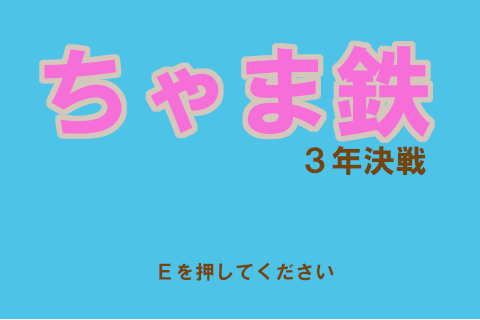
\includegraphics[scale=2.0]{sp4.png}
        \caption{タイトル画面}
         \label{title}
        \end{figure}

    図\ref{rule1}~図\ref{rule4}にルール説明画面を示す.タイトル画面でEキーを押すとはじめに
    図\ref{rule1}の画面が表示される.図\ref{rule1}の状態でEキーを押すと図\ref{rule2}の画面が
    表示される.図\ref{rule3}の場合も同様である.図\ref{rule4}の場合でEキーを押すまたは,Sキーを押した場合,
    次節で示す目的地の設定が行われる.

    \begin{figure}[H]
        \centering
        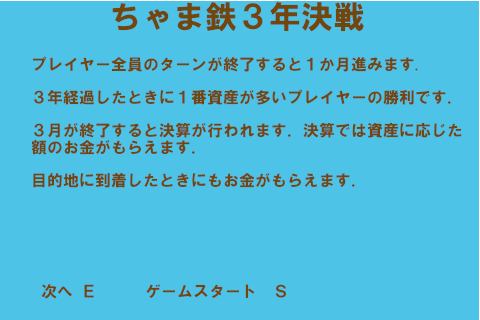
\includegraphics[scale=2.0]{sp5.png}
        \caption{ルール説明1}
         \label{rule1}
        \end{figure}
    \begin{figure}[H]
        \centering
        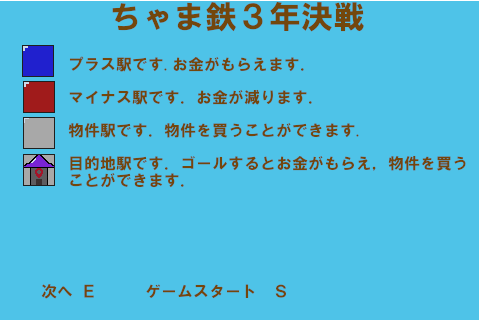
\includegraphics[scale=2.0]{sp6.png}
        \caption{ルール説明2}
         \label{rule2}
        \end{figure}
    \begin{figure}[H]
        \centering
        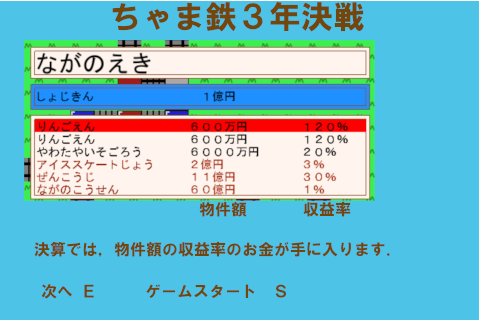
\includegraphics[scale=2.0]{sp7.png}
        \caption{ルール説明3}
         \label{rule3}
        \end{figure}
    \begin{figure}[H]
        \centering
        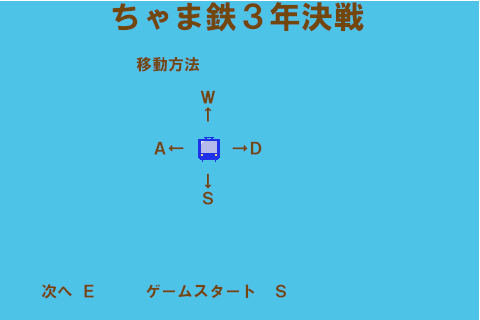
\includegraphics[scale=2.0]{sp8.png}
        \caption{ルール説明4}
         \label{rule4}
        \end{figure}
    \subsection{目的地を決める処理}
    \subsection{サイコロをふる処理}
    \subsection{駅の移動とマップの描画}
    \subsection{物件の購入処理}
    \subsection{プラス駅の処理}
    \subsection{マイナス駅の処理}
    \subsection{借金の処理}
    \subsection{ターン終了処理}
    \subsection{決算および最終成績の処理}
    \subsection{ゲーム終了処理}
    \section{感想}

    \section{ソースコード}


        \begin{thebibliography}{9}
          \bibitem{mmtt}  桃太郎電鉄,\url{https://www.konami.com/games/momotetsu/teiban/} ,閲覧日2021年1月5日
          \end{thebibliography}
\end{document}

